\chapter{Metodologia}\label{metodologia}

Neste capítulo é apresentada a metodologia utilizada para a
realização da pesquisa e contribuição tecnológica. A principal questão
a ser respondida é: se a evolução do design da apresentação dos dados do Mezuro
é suficiente para melhorar a sua visualização? Caso não, quais técnicas e
tipos de VS são mais adequadas a exibição das métricas do Mezuro?

% TODO: relembrar o que foi dito na introdução

% TODO: explicar a pergunta, "isso pq o mezuro..."

\section{Análise Exploratória do Mezuro}

% TODO: contextualizar..
% "para responder a questão, a primeira análise exploratória com os objetivos
% de fazer isso e aquilo, relaiz"

A análise exploratória do funcionamento prático do Mezuro, com os softwares do
SPB, foi realizada da seguinte forma:

% TODO: explicar estas atividades
% explicar o que eu fiz na tabela, categorizar por software
% explicar o pq dos arquivos compactados
% explicar pq a escolha do github

\begin{description}

  \item [Categorização dos softwares do SPB:]
    A categorização foi realizada em uma planinha e está disponível para
    visualização pública\footnote{\url{https://goo.gl/fYzY84}}. Foram
    catalogados apenas os softwares categorizados como \textbf{software público}.
    A ordem das linhas da planilha está por nome dos softwares, alfabeticamente.
    Além dessa coluna com os nomes, foi adicionado uma para registrar se os
    administradores do software disponibilizaram o código de forma versionada no
    Gitlab do SPB. A terceira coluna refere-se a linguagem de programação
    predominante no desenvolvimento do projeto. A coluna com o título
    \textit{Link - Código} representa o link para o espelho do código criado no
    Github. As duas últimas colunas são para o registro dos links para a
    avaliação do software no Mezuro e no CodeClimate.

  \item [Download e versionamento dos que apenas possuem o código compactado no SPB:]
    Grande parte dos softwares do SPB não possui o código-fonte versionado. Para
    a solução desse desafio, foi realizado o download dos arquivos compactados
    (zip, tar, tar.gz) dos projetos em PHP, iniciado um repositório Git no
    diretório do projeto e realizado um \textit{commit} inicial com a adição de
    todo o projeto.

  \item [Criação de um espelho no Github, em uma organização chamada \textit{spb-metrics}:]
    Após o Download e versionamento do código, foi realizada a atualização de um
    repositório remoto no Github, na organização criada específica para esta
    análise exploratória. A escolha de utilizar o Github justifica-se pelas
    limitações de inserções de projetos para avaliação no CodeClimate.
    Inicialmente, foi-se pensado o \textit{upload} em outros serviços, como o
    Bitbucket, visto que alguns softwares já possuem espelhos neste serviço.
    Porém, esta primeira abordagem foi abandonada, pois se o projeto não
    estiver disponível no Github, o CodeClimate exige uma conta paga para a
    avaliação.

    Para os softwares que possuem o código versionando no SPB, além desta
    limitação do CodeClimate, um problema com o certificado de segurança
    impossibilita o \textit{clone} de projetos utilizando o protocolo HTTPS, que
    é geralmente a forma como as ferramentas de avaliação de código-fonte faz o
    download dos softwares. Portanto, foi realizado a atualização de um outro
    espelho remoto também no Github, na organização
    \textit{spb-metrics}\footnote{\url{https://github.com/spb-metrics}}.

  \item [Adição dos softwares no Mezuro, utilizando as configurações para novas
  linguagens avaliadas por esta ferramenta]:
    \begin{itemize}
        \item Configuração do Mezuro para PHP: CodeClimate
              PHPMD\footnote{\url{http://mezuro.org/pt/kalibro\_configurations/18}}
      \item Configuração do Mezuro para Python:
              Python\footnote{\url{http://mezuro.org/pt/kalibro\_configurations/8}}
    \end{itemize}

    Após a criação do espelho no Github, foi realizado a adição destes projetos
    para a avaliação no Mezuro. Atividade esta em que foi estabelecido os
    seguintes passos:
    \begin{enumerate}
        \item Adicionado o nome utilizando o mesmo do SPB;
        \item Adicionado a descrição com a breve descrição do projeto no SPB;
        \item Para a escolha da licença, foi estabelecido utilizar a mesmo do
              software, quando possuía. Caso contrário, a escolha foi a
              \textit{Affero GNU Public License (AGPL-3.0)};
        \item Adicionado o endereço do projeto na organização
              \textit{spb-metrics} no Github;
        \item A ramo de desenvolvimento escolhido foi o principal (master);
        \item Não foi estabelecido uma frequência de reprocessamento
              \textit{(Not Periodically)};
        \item E finalmente, para a configuração, foi escolhido uma das duas
              acima citadas (ou CodeClimate PHPMD, ou Python).
    \end{enumerate}

  \item [Comparação direta com o CodeClimate]
    Para a comparação direta com a CodeClimate, foi realizado a adição dos
    projetos para a avaliação, bastando informar o nome do repositório no Github,
    por exemplo: spb-metrics/xemele, ou spb-metrics/cocar, etc. A Figura XYZ
    mostra este formulário para a importação de um repositório e análise no
    CodeClimate. Basta informar o nome do repositório; a própria ferramenta
    identifica qual a linguagem predominante e organiza as \textit{engines}
    necessárias para a coleta e análise das métricas.

  \item [Pesquisa via questionário com usuários do Mezuro:]
  ...
  \item [Especificação de Melhorias de Design da apresentação dos dados do Mezuro:]
  ...
  \item [Pré-seleção e especificação de VS para o Mezuro:]
  ...

\end{description}

\begin{comment}

\section{Pré-seleção de Visualizações}

% TODO: "o segundo passo foi então..."

A atividade de contribuição tecnológica tem como objetivo selecionar métricas
com um certo nível  de similaridade e importância quando unidas, e a exibição de
tais por meio de uma das técnicas de visualização estudadas. Esta exibição
poderá ser uma nova página ou passo dentro do fluxo percorrido pelo usuário ao
utilizar o Mezuro para o monitoramento do código, ou ainda estar contida nas
informações gerais dos repositórios registrados na plataforma.

As etapas que serão seguidas para elaboração desta atividade estão descritas
nos itens abaixo e a Figura \ref{fig:metodotologia_atividades} ilustra o
encadeamento destas etapas:

\begin{figure}[h]
  \centering
    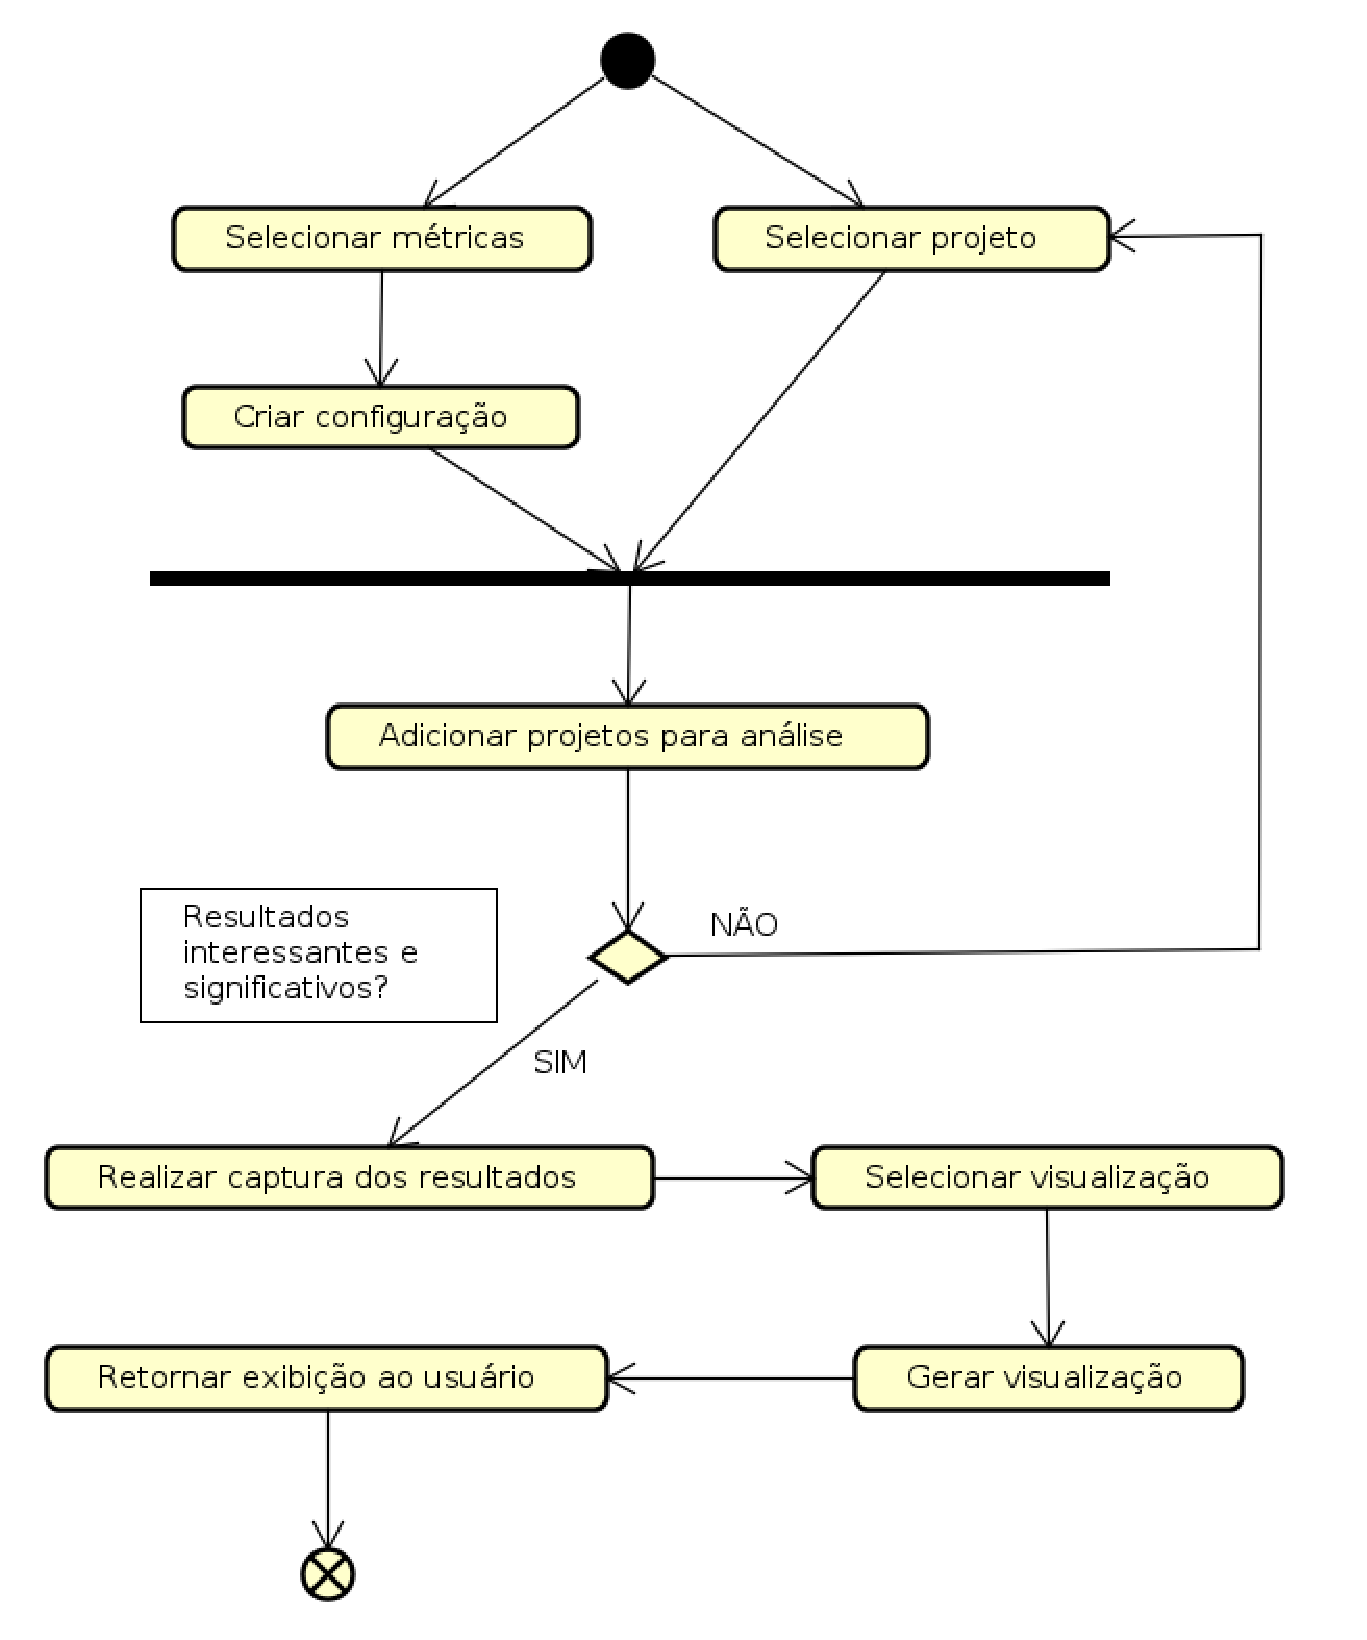
\includegraphics[keepaspectratio=true,scale=0.5]
    {figuras/metodotologia_atividades.eps}
  \caption{Encadeamento das etapas da atividade de contribuição tecnológica}
  \label{fig:metodotologia_atividades}
\end{figure}

% TODO: mudar estas atividades

\begin{enumerate}
  \item \textbf{Selecionar Configurações}: Selecionar as métricas com maior nível de
  similaridade e afinidade com os objetivos de qualidade conhecidos.

  \item \textbf{Criar configuração}: Criar o contêiner no qual as métricas
  selecionadas estarão presentes. A configuração servirá para a associação aos
  projetos selecionados e a abstração de alto nível da visualização desejada.
  Seja essa criação em ambiente de desenvolvimento, seja no próprio Mezuro em
  produção.

  \item \textbf{Selecionar projetos}: Selecionar quais projetos que melhor se
  adéquem às métricas selecionadas e/ou possivelmente forneçam dados
  interessantes e significativos para a geração da visualização. Por exemplo:
  se as métricas selecionadas forem específicas de terminada linguagem, os
  projetos devem necessariamente ter seus códigos com maioria da escrita
  nessa linguagem. O número ideal é de três projetos, podendo conter a
  combinação entre projetos que são reconhecidos por possuírem uma boa
  organização com outros que são reconhecidos por não possuírem determinado
  nível de qualidade.

  \item \textbf{Adicionar projetos para análise}: Adicionar projetos como um
  novo repositório para análise na plataforma Mezuro.

  \item \textbf{Realizar captura dos resultados}: Uma vez que os resultados
  forem interessantes e significativos, será feita a captura (parser) desses
  dados utilizando talvez as Ruby Gems Sinatra ou Seed\_dump.

  \item \textbf{Selecionar visualização}: Antes de gerar a visualização, será
  feito a escolha da melhor visualização dado o contexto, relevância e
  granularidade dos dados resultantes da análise. Levando em consideração também
  as técnicas estudadas e um número finito pré-estabelecidos de visualizações.

  \item \textbf{Gerar visualização}: utilizar biblioteca de criação de
  visualização para criação da representação alternativa dos dados da análise.

  \item \textbf{Retornar exibição ao usuário}: Nesta fase será elaborada o
  retorno da visualização ao usuário, como mencionado antes, seja em uma nova
  página ou nas informações gerais do repositório analisado.
\end{enumerate}

% TODO: talvez as etapas relacionadas ao mezuro possam estar em um único passo. Por exemplo a atividade de "Criar configuração" que são apenas alguns cliques, ou apenas um comando no console.

\section{Seleção das Métricas}

% TODO: preciso definir as métricas agora?

% TODO: selecionar métricas com certo nível de similaridade.

% TODO: explique que, devido à comodidade em já ter algumas configurações pré-estabelicidas
% no Mezuro, e dado as limitações de tempo e escopo, não poderei passar por toda uma
% "Seleção das Métricas"
% SOLUÇÃO: explicar quais são essas configurações presentes por default no Mezuro

\section{Seleção dos Projetos}

% TODO: escrever um pouco sobre os projetos para geração das VS.
% Já tenho utilizado a Engine de IJE do professor Edson Alves como parâmetro.
% O professor Paulo sugeriu o Colab, dado o grande número de contribuições que ele atingiu nos
% últimos meses por conta do SPB.

% TODO: Mudar metodologia para abranger a análise exploratória e como ela foi realizada:
%   - Prioridades na escolha dos projetos
%   - Categorização nas planilhas
%   - Disponibilizar o códio em algum  sistema de versionamento
%   - Adicionar à ferramentas: CodeClimate e Mezuro.

\end{comment}

% TODO: fechar metodologia, para não terminar com itemize
